\documentclass[12pt]{article}
\usepackage{amsmath}
\usepackage{amsfonts}
\usepackage{amssymb}
\usepackage{graphicx}
\usepackage{tikz}
\usepackage{pgfplots}
\pgfplotsset{compat=1.17}
\usepackage{array}
\usepackage{booktabs}
\usepackage{hyperref}
\usepackage{geometry}
\geometry{margin=2.5cm}
\usepackage{xepersian}
\settextfont[Path="./", Extension=".ttf"]{XB-Niloofar}
\setdigitfont[Path="./", Extension=".ttf"]{XB-Niloofar}

\begin{document}
	
	\title{تبدیل داده‌ها برای مقابله با نقاط پرت}
	\author{محمدمهدی شریف بیگی}
	\date
	\maketitle
	
	\section{مقدمه}
	
	تبدیل داده‌ها (\lr{Data Transformation}) یکی از روش‌های مؤثر برای کاهش تأثیر نقاط پرت (Outliers) است. این روش با اعمال تبدیل ریاضی مناسب، مقیاس داده‌ها را تغییر داده و توزیع آن‌ها را به شکل طبیعی‌تر درآورده و تأثیر مقادیر افرطی را کاهش می‌دهد.
	
	\section{۱. تبدیل لگاریتمی (\lr{Logarithmic Transformation})}
	
	\subsection{فرمول:}
	$$y = \log(x) \quad \text{یا} \quad y = \log_{10}(x) \quad \text{یا} \quad y = \ln(x)$$
	
	\subsection{توضیح مفصل:}
	
	تبدیل لگاریتمی یکی از پرکاربردترین روش‌های تبدیل داده است که به خصوص برای داده‌های دارای \textbf{چولگی راست} (right-skewed) بسیار مؤثر است.
	
	\subsubsection{خصوصیات ریاضی:}
	
	برای $x > 0$، تابع لگاریتم دارای خصوصیات زیر است:
	\begin{align}
		\frac{d}{dx}\ln(x) &= \frac{1}{x} \\
		\lim_{x \to \infty} \frac{\ln(x)}{x} &= 0 \\
		\ln(ab) &= \ln(a) + \ln(b)
	\end{align}
	
	این خصوصیات نشان می‌دهد که:
	\begin{itemize}
		\item شیب تابع با افزایش $x$ کاهش می‌یابد
		\item رشد لگاریتم نسبت به $x$ کندتر می‌شود
		\item ضرب در جمع تبدیل می‌شود
	\end{itemize}
	
	\subsubsection{مثال عملی با محاسبات کامل:}
	
	فرض کنید داده‌های اصلی درآمد (میلیون ریال): $\{1, 10, 100, 1000, 10000\}$
	\textbf{ مقایسه آمارهای توصیفی}
	
	\begin{center}
		\begin{tabular}{lcc}
			\toprule
			آماره & داده اصلی & داده تبدیل شده \\
			\midrule
			میانگین & \lr{$\frac{1+10+100+1000+10000}{5} = 2222.2$} & \lr{$\frac{0+1+2+3+4}{5} = 2$} \\
			میانه & \lr{$100$} & \lr{$2$} \\
			انحراف معیار & \lr{$4499.4$} & \lr{$1.58$} \\
			محدوده & \lr{$10000-1 = 9999$} & \lr{$4-0 = 4$} \\
			ضریب تغییرات & \lr{$\frac{4499.4}{2222.2} = 2.025$} & \lr{$\frac{1.58}{2} = 0.79$} \\
			\bottomrule
		\end{tabular}
	\end{center}
	
	\subsection{نمودار مقایسه‌ای بهبود یافته:}
	
	\begin{center}
		\begin{tikzpicture}[scale=0.8]
			% نمودار داده‌های اصلی
			\begin{scope}
				\draw[->] (0,0) -- (11,0) node[right] {\rl{مقدار (هزار واحد)}};
				\draw[->] (0,0) -- (0,4) node[above] {فراوانی};
				
				% داده‌های چوله راست
				\draw[fill=red!30, draw=red] (0.5,0) rectangle (1.5,3);
				\draw[fill=red!30, draw=red] (1.5,0) rectangle (2.5,2.5);
				\draw[fill=red!30, draw=red] (2.5,0) rectangle (3.5,1.8);
				\draw[fill=red!30, draw=red] (4,0) rectangle (5,1.2);
				\draw[fill=red!30, draw=red] (9,0) rectangle (10,0.5);
				
				% برچسب‌ها
				\foreach \x in {1,2,3,4,5,10}
				\draw (\x,0) -- (\x,-0.1) node[below, font=\tiny] {\x};
				\foreach \y in {1,2,3}
				\draw (0,\y) -- (-0.1,\y) node[left, font=\tiny] {\y};
				
				\node[below] at (5.5,-1) {\textbf{\rl{داده‌های اصلی (چولگی راست)}}};
			\end{scope}
			
			% نمودار داده‌های تبدیل شده
			\begin{scope}[shift={(0,-6)}]
				\draw[->] (0,0) -- (11,0) node[right] {\rl{مقدار لگاریتمی}};
				\draw[->] (0,0) -- (0,4) node[above] {فراوانی};
				
				% توزیع نرمال‌تر
				\draw[fill=blue!30, draw=blue] (1,0) rectangle (2,1.5);
				\draw[fill=blue!30, draw=blue] (3,0) rectangle (4,2.2);
				\draw[fill=blue!30, draw=blue] (5,0) rectangle (6,2.8);
				\draw[fill=blue!30, draw=blue] (7,0) rectangle (8,2.2);
				\draw[fill=blue!30, draw=blue] (9,0) rectangle (10,1.5);
				
				% برچسب‌ها
				\foreach \x in {0,1,2,3,4}
				\draw ({2*\x+1.5},0) -- ({2*\x+1.5},-0.1) node[below, font=\tiny] {\x};
				\foreach \y in {1,2,3}
				\draw (0,\y) -- (-0.1,\y) node[left, font=\tiny] {\y};
				
				\node[below] at (5.5,-1) {\textbf{\rl{داده‌های تبدیل شده (نرمال)}}};
			\end{scope}
		\end{tikzpicture}
	\end{center}
	
	\section{۲. تبدیل رادیکال (\lr{Square Root Transformation})}
	
	\subsection{فرمول:}
	$$y = \sqrt{x}$$
	
	\subsection{توضیح مفصل:}
	
	تبدیل رادیکال نسبت به تبدیل لگاریتمی ملایم‌تر است و برای داده‌هایی که دارای چولگی متوسط هستند مناسب است.
	
	\subsubsection{خصوصیات ریاضی:}
	
	برای $x \geq 0$:
	\begin{align}
		\frac{d}{dx}\sqrt{x} &= \frac{1}{2\sqrt{x}} \\
		\lim_{x \to 0^+} \frac{1}{2\sqrt{x}} &= +\infty \\
		\lim_{x \to \infty} \frac{1}{2\sqrt{x}} &= 0
	\end{align}
	
	\subsubsection{مثال عملی با محاسبات کامل:}
	
	فرض کنید داده‌های اصلی مساحت (متر مربع): $\{4, 16, 64, 256, 1024\}$
	\textbf{محاسبه دقیق آمارهای توصیفی}
	
	برای داده‌های اصلی: $X = \{4, 16, 64, 256, 1024\}$
	$$\bar{X} = \frac{4+16+64+256+1024}{5} = \frac{1364}{5} = 272.8$$
	
	$$s_X^2 = \frac{\sum(x_i - \bar{x})^2}{n-1} = \frac{(4-272.8)^2 + \cdots + (1024-272.8)^2}{4}$$
	
	$$s_X^2 = \frac{72267.04 + 66022.24 + 43436.84 + 379.24 + 564840.64}{4} = \frac{746946}{4} = 186736.5$$
	
	$$s_X = \sqrt{186736.5} = 432.01$$
	
	برای داده‌های تبدیل شده: $Y = \{2, 4, 8, 16, 32\}$
	$$\bar{Y} = \frac{2+4+8+16+32}{5} = \frac{62}{5} = 12.4$$
	
	$$s_Y^2 = \frac{(2-12.4)^2 + (4-12.4)^2 + (8-12.4)^2 + (16-12.4)^2 + (32-12.4)^2}{4}$$
	
	$$s_Y^2 = \frac{108.16 + 70.56 + 19.36 + 12.96 + 384.16}{4} = \frac{595.2}{4} = 148.8$$
	
	$$s_Y = \sqrt{148.8} = 12.2$$
	
	\subsection{نمودار تابع رادیکال:}
	
	\begin{center}
		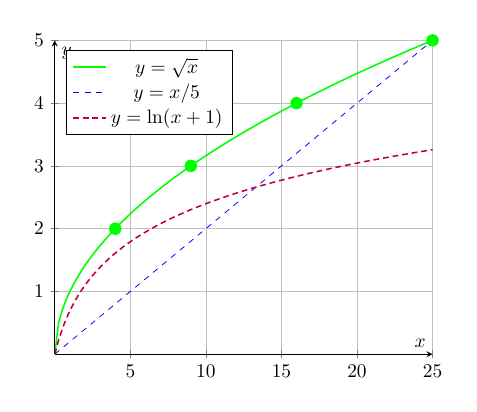
\begin{tikzpicture}[scale=0.7]
			\begin{axis}[
				axis lines = center,
				xlabel = {$x$},
				ylabel = {$y$},
				domain = 0:25,
				samples = 100,
				grid = major,
				legend pos = north west
				]
				\addplot[green, thick] {sqrt(x)};
				\addplot[blue, dashed] {x/5};
				\addplot[purple, thick, densely dashed] {ln(x+1)};
				
				\legend{\lr{$y = \sqrt{x}$}, \lr{$y = x/5$}, \lr{$y = \ln(x+1)$}}
				
				% نقاط خاص
				\addplot[only marks, mark=*, mark size=3pt, green] coordinates {(4,2) (9,3) (16,4) (25,5)};
			\end{axis}
		\end{tikzpicture}
	\end{center}
	
	\section{۳. تبدیل باکس-کاکس (\lr{Box-Cox Transformation})}
	
	\subsection{فرمول:}
	$$y = \begin{cases}
		\frac{x^{\lambda} - 1}{\lambda} & \text{اگر } \lambda \neq 0 \\
		\ln(x) & \text{اگر } \lambda = 0
	\end{cases}$$
	
	\subsection{تفسیر ریاضی مقادیر مختلف $\lambda$:}
	
	\subsubsection{$\lambda = 2$ (تبدیل درجه دوم):}
	$$y = \frac{x^2 - 1}{2}$$
	
	این تبدیل برای داده‌هایی که چولگی چپ دارند (left-skewed) مناسب است.
	
	\subsubsection{$\lambda = 1$ (تبدیل خطی):}
	$$y = x - 1$$
	
	این تبدیل فقط یک انتقال ساده است و شکل توزیع را تغییر نمی‌دهد.
	
	\subsubsection{$\lambda = 0.5$ (تبدیل رادیکال):}
	$$y = \frac{\sqrt{x} - 1}{0.5} = 2(\sqrt{x} - 1)$$
	
	\subsubsection{$\lambda = 0$ (تبدیل لگاریتمی):}
	$$y = \ln(x)$$
	
	\subsubsection{$\lambda = -0.5$ (تبدیل معکوس رادیکال):}
	$$y = \frac{x^{-0.5} - 1}{-0.5} = 2\left(1 - \frac{1}{\sqrt{x}}\right)$$
	
	\subsubsection{$\lambda = -1$ (تبدیل معکوس):}
	$$y = 1 - \frac{1}{x}$$
	
	\subsection{روش یافتن $\lambda$ بهینه:}
	
	پارامتر $\lambda$ از طریق بیشینه‌سازی تابع درستنمایی محاسبه می‌شود:
	
	$$L(\lambda) = -\frac{n}{2}\ln\left(\frac{\text{RSS}(\lambda)}{n}\right) + (\lambda-1)\sum_{i=1}^{n}\ln(x_i)$$
	
	که در آن:
	\begin{align}
		\text{RSS}(\lambda) &= \sum_{i=1}^{n}\left[y_i(\lambda) - \bar{y}(\lambda)\right]^2 \\
		y_i(\lambda) &= \begin{cases}
			\frac{x_i^{\lambda} - 1}{\lambda} & \lambda \neq 0 \\
			\ln(x_i) & \lambda = 0
		\end{cases}
	\end{align}
	
	\textbf{الگوریتم محاسبه:}
	\begin{enumerate}
		\item مقادیر مختلف $\lambda$ را در بازه $[-2, 2]$ با گام $0.1$ آزمایش کنید
		\item برای هر $\lambda$، داده‌ها را تبدیل کنید
		\item $L(\lambda)$ را محاسبه کنید
		\item $\lambda$ که بیشترین $L(\lambda)$ را دارد، انتخاب کنید
	\end{enumerate}
	
	\subsection{مثال عملی کامل:}
	
	داده‌های اصلی: $\{9, 25, 100, 400\}$، فرض کنید $\lambda = 0.5$ بهینه محاسبه شده است.
	
	\textbf{گام ۱: تبدیل داده‌ها}
	\begin{align}
		y_1 &= \frac{9^{0.5} - 1}{0.5} = \frac{3 - 1}{0.5} = \frac{2}{0.5} = 4 \\
		y_2 &= \frac{25^{0.5} - 1}{0.5} = \frac{5 - 1}{0.5} = \frac{4}{0.5} = 8 \\
		y_3 &= \frac{100^{0.5} - 1}{0.5} = \frac{10 - 1}{0.5} = \frac{9}{0.5} = 18 \\
		y_4 &= \frac{400^{0.5} - 1}{0.5} = \frac{20 - 1}{0.5} = \frac{19}{0.5} = 38
	\end{align}
	
	\textbf{گام ۲: محاسبه آمارهای توصیفی}
	
	داده‌های اصلی: میانگین = $\frac{9+25+100+400}{4} = 133.5$، انحراف معیار = $181.9$
	
	داده‌های تبدیل شده: میانگین = $\frac{4+8+18+38}{4} = 17$، انحراف معیار = $15.6$
	
	ضریب تغییرات کاهش یافته: از $\frac{181.9}{133.5} = 1.36$ به $\frac{15.6}{17} = 0.92$
	
	\subsection{نمودار اثر مقادیر مختلف $\lambda$:}
	
	\begin{center}
		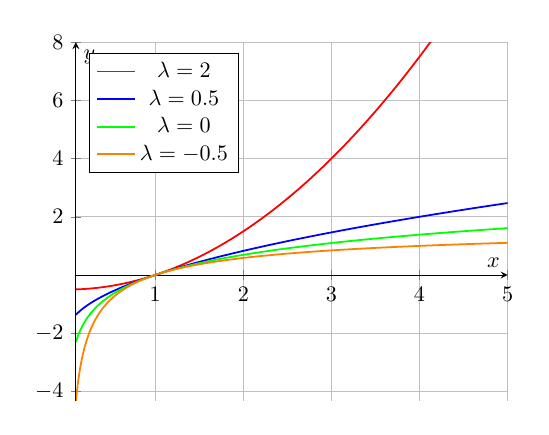
\begin{tikzpicture}[scale=0.8]
			\begin{axis}[
				axis lines = center,
				xlabel = {$x$},
				ylabel = {$y$},
				domain = 0.1:5,
				samples = 200,
				grid = major,
				legend pos = north west,
				ymax = 8
				]
				
				% λ = 2
				\addplot[red, thick] {(x^2 - 1)/2};
				
				% λ = 0.5
				\addplot[blue, thick] {2*(sqrt(x) - 1)};
				
				% λ = 0 (log)
				\addplot[green, thick] {ln(x)};
				
				% λ = -0.5
				\addplot[orange, thick] {2*(1 - 1/sqrt(x))};
				
				\legend{\lr{$\lambda = 2$}, \lr{$\lambda = 0.5$}, \lr{$\lambda = 0$}, \lr{$\lambda = -0.5$}}
			\end{axis}
		\end{tikzpicture}
	\end{center}
	
	\section{مقایسه کمی سه روش}
	
	\subsection{مثال کاربردی: داده‌های درآمد}
	
	داده‌های درآمد (میلیون تومان): $\{2, 5, 8, 12, 15, 25, 45, 120\}$
	
	\subsubsection{محاسبات دقیق:}
	
	\textbf{۱. آمارهای اصلی:}
	\begin{align}
		\bar{x} &= \frac{2+5+8+12+15+25+45+120}{8} = \frac{232}{8} = 29 \\
		s^2 &= \frac{\sum(x_i - 29)^2}{7} = \frac{11914}{7} = 1702 \\
		s &= \sqrt{1702} = 41.26 \\
		\text{چولگی} &= \frac{\sum(x_i - 29)^3/8}{s^3} = 1.89
	\end{align}
	
	\textbf{۲. تبدیل لگاریتمی:}
	$$y_{\text{log}} = \{\ln(2), \ln(5), \ln(8), \ln(12), \ln(15), \ln(25), \ln(45), \ln(120)\}$$
	$$= \{0.69, 1.61, 2.08, 2.48, 2.71, 3.22, 3.81, 4.79\}$$
	
	میانگین: $\bar{y}_{\text{log}} = 2.67$، انحراف معیار: $s_{\text{log}} = 1.35$، چولگی: $0.23$
	
	\textbf{۳. تبدیل رادیکال:}
	$$y_{\text{sqrt}} = \{\sqrt{2}, \sqrt{5}, \sqrt{8}, \sqrt{12}, \sqrt{15}, \sqrt{25}, \sqrt{45}, \sqrt{120}\}$$
	$$= \{1.41, 2.24, 2.83, 3.46, 3.87, 5.00, 6.71, 10.95\}$$
	
	میانگین: $\bar{y}_{\text{sqrt}} = 4.56$، انحراف معیار: $s_{\text{sqrt}} = 3.24$، چولگی: $0.67$
	
	\begin{center}
		\begin{tabular}{lccc}
			\toprule
			\textbf{آماره} & \textbf{داده اصلی} & \textbf{لگاریتمی} & \textbf{رادیکال} \\
			\midrule
			میانگین & ۲۹.۰ & ۲.۶۷ & ۴.۵۶ \\
			انحراف معیار & ۴۱.۲۶ & ۱.۳۵ & ۳.۲۴ \\
			ضریب تغییرات & ۱.۴۲ & ۰.۵۱ & ۰.۷۱ \\
			چولگی & ۱.۸۹ & ۰.۲۳ & ۰.۶۷ \\
			\bottomrule
		\end{tabular}
	\end{center}
	
	\section{راهنمای عملی انتخاب روش}
	
	\subsection{الگوریتم تصمیم‌گیری علمی:}
	
	\begin{enumerate}
		\item \textbf{محاسبه ضریب چولگی ($\gamma_1$):}
		$$\gamma_1 = \frac{E[(X-\mu)^3]}{\sigma^3} = \frac{\sum_{i=1}^{n}(x_i - \bar{x})^3/n}{s^3}$$
		
		\item \textbf{قانون تصمیم‌گیری:}
		\begin{itemize}
			\item اگر \lr{$|\gamma_1| < 0.5$}: نیازی به تبدیل نیست
			\item اگر \lr{$0.5 \leq |\gamma_1| < 1$}: تبدیل رادیکال
			\item اگر \lr{$|\gamma_1| \geq 1$}: تبدیل لگاریتمی یا باکس-کاکس
		\end{itemize}
		
		\item \textbf{آزمون نرمالیتی شاپیرو-ویلک:}
		$W = \frac{\left(\sum_{i=1}^{n} a_i x_{(i)}\right)^2}{\sum_{i=1}^{n} (x_i - \bar{x})^2}$
		
		اگر \lr{$p\text{-value} > 0.05$}، داده‌ها نرمال هستند.
	\end{enumerate}
	
	\section{نتیجه‌گیری}
	
	تبدیل داده‌ها ابزار قدرتمندی برای مقابله با نقاط پرت و بهبود نرمالیتی است. انتخاب روش مناسب باید بر اساس:
	
	\begin{itemize}
		\item تحلیل کمی چولگی داده‌ها
		\item آزمون‌های آماری نرمالیتی
		\item ماهیت علمی متغیرها
		\item هدف نهایی تحلیل
	\end{itemize}
	
	همیشه قبل و بعد از تبدیل، آزمون‌های آماری مناسب را انجام دهید تا از مؤثر بودن تبدیل اطمینان حاصل کنید.
	
\end{document}